\section{Theorie}
\label{sec:Theorie}

\subsection{Einleitung}

Innerhalb dieses Experiments werden diverse Messungen mit Hilfe eines Helium-Neon Lasers
durchgeführt um ein besseres Verständnis von diesem zu bekommen. Darunter zählen unter anderem
eine Polarisationsmessung, eine Doppelspaltmessung, mehrere Ausmessungen im Laser entstehender
Moden und eine Stabilitätsmessung.
Dazu werden zunächst theoretische Grundlagen zu Lasern im Allgemeinen, auftretende
elektomagnetische Moden und der speziellen Funktionsweise des Helium-Neon Lasers erläutert
und im Anschluss daran der Aufbau und die Durchführung dieses Experiments beschrieben.
Darauffolgend präsentieren wir unsere Ergebnisse in der Auswertung und diskutieren diese
anschließend.

\subsection{Funktionsweise eines Lasers}

Die wesentliche Eigenschaft eines Lasers ist, dass er mit Hilfe von stimulierter
Emission in der Lage ist, monochromatisches Licht mit hoher Intensität und
hoher Kohärenz zu erzeugen.
Um einen Laser zu realisieren werden im Allgemeinen drei Komponenten benötigt:
eine Pumpquelle, ein Lasermedium und ein Resonator. Im Lasermedium muss durch die zugeführte
Energie der Pumpquelle eine Besetzungsinversion induziert werden können
damit der Laser überhaupt funktionieren kann. Um dies genauer zu verstehen,
werden im folgenden Abschitt zunächst verschiedene Arten von Emission und Absorption
anhand eines Zweiniveausystems erklärt.

Im thermodynamischen Gleichgewicht und ohne äußere Energiezufuhr ist der Grundzustand im
Zweiniveausystem stärker besetzt als der angeregte Zustand. Pumpt man Photonen mit einer Energie,
die der Energiedifferenz der beiden Niveaus entspricht, in das System, so werden diese mit der Rate
\begin{align}
  \frac{\mathrm{d}{N}_A}{\mathrm{d}t} = n_1 \rho(\nu) B_{12}
\end{align}
absorbiert, wobei ein Elektron vom Grundzustand in den angeregten Zustand angehoben wird. Dabei ist $n_1$
die Besetzungszahl des Grundzustands, $\rho(\nu)$ das Strahlungsfeld und $B_{12}$ ein sogenannter
Einsteinkoeffizient. Andersherum kann ein Elektron auch unter Emission eines Photons vom angeregten
Zustand in den Grundzustand übergehen. Dabei wird zwischen spontaner Emission, die unabhängig vom
externen Strahlungsfeld auftritt gemäß der Rate
\begin{align}
  \frac{\mathrm{d}{N}_\text{spont}}{\mathrm{d}t} = n_2 A_{21},
\end{align}
und induzierter Emission, deren Rate
\begin{align}
  \frac{\mathrm{d}{N}_\text{ind}}{\mathrm{d}t} = n_2 \rho(\nu) B_{21}
\end{align}
proportional zum Strahlungsfeld ist, unterschieden. Bei der spontanen Emission werden Photonen in beliebige
Richtung und beliebiger Phase emittiert, während bei der induzierten Emission Phase und Richtung von einfallendem
Photon und ausfallenden Photonen übereinstimmen. Alle drei beschriebenen Fälle sind in Abbildung
\ref{fig:absemi} skizziert. Sind die Zustände des Zweiniveausystems nicht entartet, so gilt für die
Einsteinkoeffizienten
\begin{align}
  B_{12} = B_{21} = B.
\end{align}
Es folgt sofort, dass in diesem System keine Besetzungsinversion erzeugt werden kann, denn die
gesamte Rate für Übergänge vom angeregten Zustand in den Grundzustand ist in jedem Fall bei
einer Besetzung von $n_1 = n_2 = 0.5$ größer, als die Rate für Übergänge in die andere Richtung.
Entsprechend ist ein Zweiniveausystem ungeeignet als Lasermedium.

\begin{figure}[H]
  \centering
  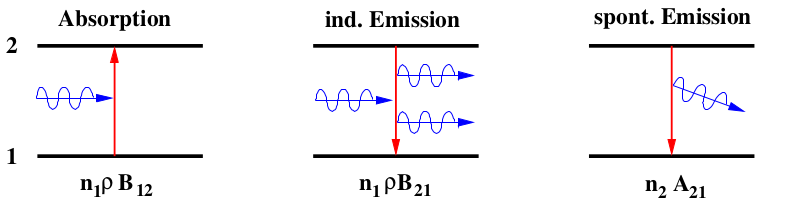
\includegraphics[height = 3.7cm]{Pics von Buddy/absemi.png}
  \caption{Strahlungsübergänge in einem Zweiniveausystem \cite{anleitung}.}
  \label{fig:absemi}
\end{figure}

Der Grund, warum eine Besetzungsinversion für das Lasen erforderlich ist, liegt darin, dass das
Strahlungsfeld sich nur dann beim Durchgang durch das Medium selbst verstärken kann.
Ein Dreiniveausystem beispielsweise, wie es in Abbildung \ref{fig:dreiniveau} zu sehen ist,
erfüllt diese Bedingung unter bestimmten Voraussetzung.
Dafür werden Elektronen vom Grundzustand in den höchst angeregten dritten Zustand gepumpt.
Eine wichtige Notwendigkeit ist, dass der anschließende Übergang vom höchsten in
den mittleren Zustand schnell geschieht, der dritte Zustand also instabil ist. Damit werden
die Elektronen letzlich indirekt vom Grundzustand in den ersten angeregten Zustand gepumpt.
Das indirekte Pumpen hat den Vorteil, dass keine Strahlungsübergänge via induzierte Emission
durch die Pump Photonen vom mittleren Niveau in den Grundzustand mehr auftreten, da die
Energiedifferenz eine andere ist. Dadurch kann erreicht werden, dass die Rate, mit welcher
das zweite Niveau befüllt wird, auch bei einer Besetzung von $n_1 = n_2 = 0.5$ noch größer
als die Rate, mit welcher der Grundzustand befüllt wird, ist und eine Besetzungsinversion
erzeugt werden. Fällt bei diesen Gegebenheiten nun ein Strahlungsfeld $\rho$ mit
der entsprechenden Photonenergie ein, so induziert dieses wegen der Besetzungsinversion mehr
Emissionen als Absorptionen, sodass es sich selbst durch das Lasermedium verstärkt.
Diese Verstärkung der Lichtintensität verläuft exponentiell mit der Strecke, die der Lichtstrahl
durch das aktive Lasermedium zurücklegt. Durch den oben bereits aufgezählten Resonator kann diese
Strecke erheblich vergrößert werden, sodass ein intensiver Laserstrahl erzeugt wird.
Wie genau das funktioniert wird im folgenden Abschnitt erläutert.

\begin{figure}[H]
  \centering
  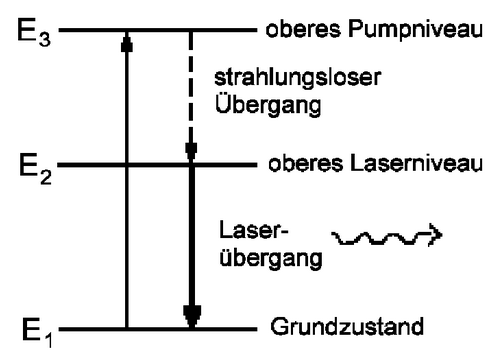
\includegraphics[height = 4.4cm]{Pics von Buddy/dreiniveau.png}
  \caption{Strahlungsübergänge in einem Dreiniveausystem \cite{laser}.}
  \label{fig:dreiniveau}
\end{figure}

Der grundlegende Aufbau eines Lasers ist in Abbildung \ref{fig:laseraufbau} erkennbar.
Zwei Spiegel, die um das Lasermedium platziert werden, reflektieren den austretenden
Lichtstrahl zurück in das Medium, wo er sich selbst verstärkt. Einer der Spiegel ist
teildurchlässig mit einem Transmissionskoeffizienten von etwa $1-2 \, \si{\percent}$,
damit der erzeugte Laserstrahl ausgekoppelt werden kann. Zusammen bilden die beiden
Spiegel einen optischen Resonator für das vom Medium emittierte Licht. Dieses genießt
abhängig von seiner Wellenlänge und der Länge des Resonators konstruktive bzw. destruktive
Interferenz. Der optische Resonator kann
prinzipiell aus planaren oder sphärischen Spiegeln bestehen, dabei muss allerdings auf
die Position der Brennpunkte geachtet werden. Werden die Resonatorparameter
\begin{align}
  g_i = 1 - \frac{L}{r_i}
\end{align}
für jeden Spiegel $i$ betrachtet, wobei $L$ die Resonatorlänge und $r_i$ der Krümmungsradius
des jeweiligen Spiegels ist, so kann hergeleitet werden, dass die Spiegel außerhalb des Intervalls
\begin{align}
  g_1 \cdot g_2 \in [0,1)
  \label{eqn:stab}
\end{align}
keinen stabilen Resonator mehr für den Lichtstrahl formen. Im Optimalfall, bei einem sogenannten
konfokalen Resonator, fallen die Brennpunkte der Spiegel genau aufeinander. Das ist nur mit
zwei sphärischen Spiegeln realisierbar, da der Brennpunkt eines planaren Spiegels im Unendlichen
liegt. Abhängig von Unebenheiten und dem Abstand zwischen den Spiegeln genießen unterschiedliche
Moden konstruktive Interferenz. Dies wird im nächsten Abschnitt genauer behandelt.

\begin{figure}
  \centering
  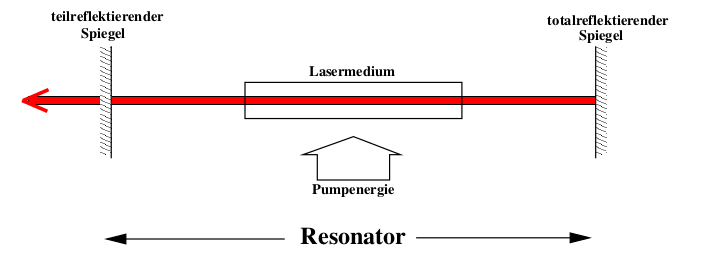
\includegraphics[height=5cm]{Pics von Buddy/laseraufbau.png}
  \caption{Schematischer Aufbau eines Lasers \cite{anleitung}.}
  \label{fig:laseraufbau}
\end{figure}

\subsection{TEM-Moden in einem Laser}

Die intuitivsten Moden, die in einem Laser entstehen können sind die longitudinalen
Moden, die sich längs der optischen Achse ausbreiten. Davon gibt es einige, da die
Wellenlänge des emittierten Lichts wesentlich geringer als die Länge des Resonators ist.
Eine Methode zur Ausmessung dieser Moden wird im nächsten Abschnitt behandelt.
Wegen Unebenheiten bei den planaren Spiegeln, oder Verkippungen bei den sphärischen o.Ä.
können aber auch transversale Moden, die sich orthogonal zur optischen Achse ausbreiten, entstehen.
Die verschiedenen auftretenden Moden werden in Anlehnung an Hohlleiter als $\text{TEM}_{lpq}$-Moden
bezeichnet. Dabei stehen $l$ und $p$ für die Anzahl an Knoten in x- und y-Richtung, also
in transversale Richtung, und $q$ für die Anzahl an Knoten in z- also longitudinale
Richtung. Für einen konfokalen Resonator mit runden Spiegeln kann die genäherte Intensitätsverteilung
für diverse TEM-Moden berechnet werden. Für die $\text{TEM}_{00}$-Mode ergibt sich damit
\begin{align}
  I(r) = I_0 \mathrm{e}^{\frac{-2 r^2}{\omega^2}}
\end{align}
wobei $I_0$ die maximale Intensität im Zentrum des Strahls und $2 \omega$ der Strahldurchmesser ist.
Diese Mode ist die intensivste mit den wenigsten Verlusten und daher auch die beobachtbare.
Eine weitere Mode, die ohne Weiteres nicht beobachtbar ist, ist die $\text{TEM}_{01}$-Mode von der Form
\begin{align}
  I(r) = I_0 r^2 \mathrm{e}^{\frac{-2 r^2}{\omega^2}}.
\end{align}
Um sie zu beobachten wird eine sogenannte Modenblende benötigt. Dazu wird in diesem Versuch ein
schmaler Wolframdraht verwendet, welcher die intensive, scharf zentrierte Grundmode optisch ausblenden soll.

\subsection{Ausmessung longitudinaler Moden mittels Fouriertransformation}
\label{sec:long}

Wie bereits erwähnt treten einige longitudinalen Moden im Laser auf, die alle mit einem Frequenz-Abstand von etwa
\begin{align}
  \Delta \nu = \frac{c}{2 L} \approx \SI{100}{\mega\hertz}
  \label{eqn:freqabstand}
\end{align}
beieinander liegen. Misst man die zeitlichen Intensitätschwankungen des Lasers durch die longitudinalen Moden
so erhält man eine Schwebung all dieser Moden, aus welcher in dieser Form keine vernünftigen Ergebnisse
abgelesen werden können. Im Fourier- oder Frequenzraum allerdings entsprechen diese Schwingungen einfach
mehreren Deltapeaks die im durch Gleichung \eqref{eqn:freqabstand} gegebenen Abstand nebeneinander positioniert sind.
Werden die Intensitätsschwankungen also mit einem FFT-Gerät einer Fouriertransformation unterzogen, so kann
ein klares Bild der Frequenzen aufgenommen werden und daraus schließlich eine experimentelle Messung der
Resonatorlänge ohne Maßband durchgeführt werden.
Nachdem in diesen beiden Abschnitten eine kurze Beschreibung der auftretenden Moden in einem Laser geliefert wurde,
wird im nächsten Abschnitt der in diesem Versuch verwendete Helium-Neon Laser vertieft.

\subsection{Funktionsweise eines Helium-Neon Laser}

Der Helium-Neon Laser ist ein Gaslaser bestehend aus einem länglichem Rohr, welches ein Gemisch aus Helium und Neon
im Verhältnis 5:1 beinhaltet und an beiden Seiten jeweils durch ein Brewsterfenster abgeschlossen wird.
Die Bedeutung der Brewsterfenster wird im nächsten Abschnitt diskutiert. Als Pumpquelle dient eine äußere
elektrische Spannung, die an den Helium-Atomen elektrische Entladungen erzeugt. Dabei wird für das rote
Laserlicht ein Elektron aus dem Helium-Grundzustand in den $2^1 s$-Zustand angehoben. Die angeregten Helium-Atome
befinden sich in metastabilen Zuständen, vergleichbar mit dem oberen Pumpniveau im Dreiniveausystem, siehe Abbildung
\ref{fig:dreiniveau}. Durch Stöße zweiter Art wird die überschüssige Energie von den Helium-Atomen auf die
Neon-Atome übertragen. Diese befinden sich dann im metastabilen $5s$-Zustand, was genau dem oberen
Laserniveau des Dreiniveausystems entspricht, vergleiche dazu Abbildung \ref{fig:dreiniveau}.
Das charakteristische rote Laserlicht mit einer Wellenlänge von etwa $\lambda = \SI{632,8}{\nano\meter}$
wird schließlich durch spontane und stimulierte Übergänge vom $5s$-Niveau in das $3p$-Niveau erzeugt.
Dadurch, dass die Neon-Atome durch die Helium-Atome indirekt angeregt werden wird im Gegensatz zu einem
Zweiniveausystem eine Besetzungsinversion induziert. In Abbildung \ref{fig:HeNeÜbergänge} sind die
aufgezählten Schritte für das Entstehen des Laserlichts noch einmal graphisch dargestellt.

\begin{figure}[H]
  \centering
  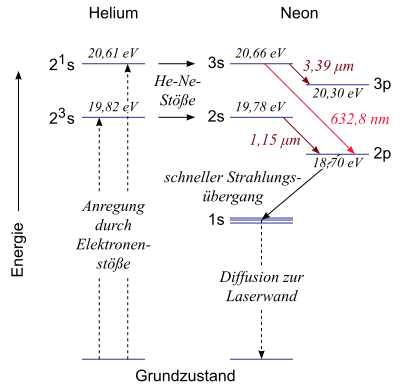
\includegraphics[height = 6.5cm]{Pics von Buddy/heneübergänge.png}
  \caption{Niveauübergänge im Helium-Neon Laser. Relevant für diesen Versuch ist nur der rote Übergang \cite{goettingen}.}
  \label{fig:HeNeÜbergänge}
\end{figure}

\subsection{Verwendung von Brewsterfenstern}

Ein weiterer wichtiger Aspekt des Lasers ist, dass das Laserrohr, welches das Gasgemisch beinhaltet,
an beiden Enden jeweils durch ein Brewsterfenster abgeschlossen ist. Diese ermöglichen einerseits
eine relativ verlustfreie Transmission und andererseits filtern sie den Laserstrahl abhängig
von dessen Polarisation. Prinzipiell hat das im Medium erzeugte Licht zwar eine feste Richtung,
ist aber unpolarisiert. Bezüglich einer Einfallsebene, die hier durch den Einstellwinkel des
Brewsterfensters gegeben ist, kann das unpolarisierte Licht in einen s-polarisierten und in einen
p-polarisierten Anteil aufgeteilt werden. Dabei ist der s-polarisierte Anteil senkrecht zur Einfallsebene, die
durch den einfallenden Lichtstrahl und (gedachtem) reflektierten Lichtstrahl am Brewsterfenster aufgespannt wird,
und der p-polarisierte Anteil parallel zu dieser. Wie in Abbildung \ref{fig:brewster} erkennbar,
wird der s-polarisierte Anteil an den Grenzflächen des Brewsterfensters teilweise reflektiert,
während der p-polarisierte Anteil vollständig transmittiert. Das s-polarisierte Licht büßt an jeder
Grenzfläche Intensität ein, sodass es schließlich nicht mehr durch stimulierte Emission selbstverstärkt
wird und dementsprechend nicht mehr zum Laserlicht beiträgt. Erwartet wird also, dass der resultierende
Laserstrahl linear, parallel zur Einfallsebene der Brewsterfenster polarisiert ist. Mit Hilfe eines
Polarisationsfilters, welcher linear polarisiertes Licht in Richtung eines bestimmten eingestellten
Winkels durchlässt, kann dieses Resultat nachgemessen werden. Um einen Zusammenhang zwischen der
Intensität des Laserstrahls in Abhängigkeit von der Polarisator-Einstellung zu erlangen, wird
zunächst der p-polarisierte Lichtstrahl bezüglich der Einstellrichtung des Polarisationsfilters in einen
parallelen und einen orthogonalen Anteil aufgespalten. Der parallele Anteil wird vollständig durchgelassen
und der orthogonale Anteil vollständig absorbiert.

\begin{figure}[H]
  \centering
  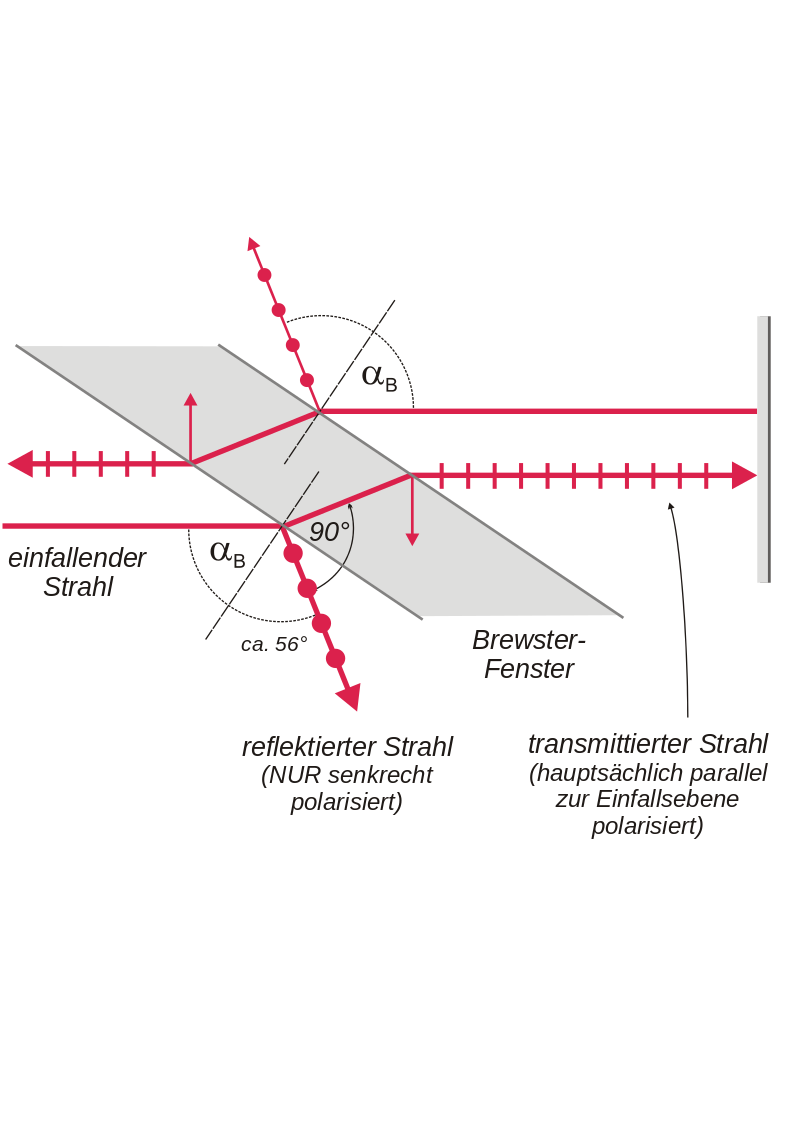
\includegraphics[height = 10.0cm]{Pics von Buddy/brewster.png}
  \caption{Strahlengang am Brewsterfenster. Die Punkte stellen die s-Polarisation dar, während die
  Striche die p-Polarisation darstellen \cite{goettingen}.}
  \label{fig:brewster}
\end{figure}

Das transmittierte E-Feld des Laserstrahls ergibt sich also
vollständig aus dem parallelen Anteil
\begin{align}
  E_{\text{pol}}(\varphi) = E_0 \cos(\varphi),
\end{align}
wobei $E_0$ das maximale Feld und $\varphi$ der relative Winkel zwischen Einfallsebene des Brewsterfensters
und Einstellrichtung des Polarisationsfilters ist. Die Intensität ergibt sich durch Quadrieren
\begin{align}
  I_{\text{pol}}(\varphi) = I_0 \cos^2(\varphi).
\end{align}
Die theoretischen Grundlagen sind damit weitestgehend behandelt. Im folgenden Kapitel
wird der Aufbau und die Durchführung für das Experiment beschrieben.
